%&pdflatex
\documentclass[11pt]{article}
\usepackage{url,enumerate, amssymb, amsfonts}
\usepackage[colorlinks = true,
linkcolor = blue,
urlcolor  = blue,
citecolor = green,
anchorcolor = blue]{hyperref}
%\usepackage{setspace,listings}
\usepackage[dvipdfmx]{graphicx}
\usepackage{amsmath}
\usepackage{psfrag}
\usepackage[font=small,labelfont=bf]{caption}
\usepackage{enumerate}
\usepackage{natbib}
\usepackage{url} % not cruci
%\pdfminorversion=4
\usepackage{setspace}
\usepackage{lscape}
\usepackage{color,amssymb}
\usepackage{mathtools}
\usepackage{dcolumn}
\usepackage{indentfirst, verbatim, float}
\usepackage[margin=0.82in]{geometry}
%\newcounter{equationset, sectsty, breqn}
%\usepackage{setspace, amsmath,color}
%\usepackage{color,amssymb}
\usepackage{mathtools, amsthm, subcaption}
\theoremstyle{definition}
\newtheorem{definition}{Definition}[section]
\newtheorem{theorem}{Theorem}[section]
\newtheorem{corollary}{Corollary}[theorem]
\newtheorem{lemma}[theorem]{Lemma}
\newtheorem{remark}{Remark}
\bibliographystyle{plainnat}
\usepackage{sidecap}
\usepackage{titlesec}
\sidecaptionvpos{figure}{c}

% NOTE: To produce blinded version, replace "0" with "1" below.
\newcommand{\blind}{1}

% DON'T change margins - should be 1 inch all around.

\begin{document}


\def\spacingset#1{\renewcommand{\baselinestretch}%
{#1}\small\normalsize} \spacingset{1}


%%%%%%%%%%%%%%%%%%%%%%%%%%%%%%%%%%%%%%%%%%%%%%%%%%%%%%%%%%%%%%%%%%%%%%%%%%%%%%

\if1\blind
{
  \title{\bf Testing independence in networks via family of network metrics}
  \author{Youjin Lee (ylee160@jhu.edu) \thanks{
    This is a joint work with Cencheng Shen (cshen6@jhu.edu) and Joshua T. Vogelstein (jovo@jhu.edu), Johns Hopkins University.}\hspace{.2cm}\\
    Department of Biostatistics, Johns Hopkins School of Publich Health}
\date{}
  \maketitle
} \fi

\if0\blind
{
  \bigskip
  \bigskip
  \bigskip
  \begin{center}
    {\LARGE\bf Testing independence in networks via family of network metrics}
\end{center}
  \medskip
} \fi

\begin{abstract}
%The text of your abstract. 200 or fewer words.
Propelled by increasing demand and supply in network data, investigating whether network structures are associated with the attributes of interest has been an important concern in natural or social science. We consider the problem of network dependence, which refers to any types of dependence between network topology and its nodal attributes and propose the method to test network independence. However due to the interdependency in constructing network, standard independence test cannot be directly applied and most of the network model-based tests presume globally persistent dependency patterns. To overcome these challenges, we propose a nonparametric multiscale test statistic which is robust to both high dimensionality and nonlinearity by utilizing a family of network geometries. Our simulation studies demonstrate the outstanding performance of the method under various circumstances. 
\end{abstract}

\noindent%
{\it Keywords:} Distance correlation, Network dependence, Diffusion maps, Exchangeable graph

\sloppy
\doublespacing

\section{Introduction}
\label{sec:intro}
	\vspace*{-0.2cm}
% suggests the research question : starts from general dependency - one variable of interest is defined over network 
Statisticians have long considered the problem of revealing the relationship between two data sets. Above all determining the existence any association or any dependence would be the first step in characterizing the relationship. As types of data have diversified or dimension of the data has increased, various forms of multivariate independence tests have been suggested~\citep{taskinen2005multivariate, heller2012consistent, szekely2007measuring}. We consider independence test upon non-traditional but ubiquitous dataset of \textit{network} which is very likely to possess the properties of both high dimensionality and nonlinearity. Network, formally defined as a collection of nodes and edges, has been suffering from a dearth of proper analysis due to its distinct way to be constructed. In this paper we define any kinds of dependency between network topology and nodal attributes as \textit{network dependence} and propose the method to test network independence. 

% literature reviews about testing network independence. 
The literature on identifying dependency between network and nodal attributes has primarily focused on their relationship explained only by network model under the boundary of model assumption \citep{wasserman1996logit, howard2016understanding}. A fundamental difficulty of model-based independence tests comes from the fact that not all networks exhibit the structures described by known network models. \cite{fosdick2015testing} overcome this issue by estimating network factors which are believed to embody each node's locations in network space. Their network models, however, still rely on the assumption that all the nodes in network would follow the same pattern of dependence -- subject to additive and multiplicative effect. 

% specify the goal / approach of our research and explain the outline 
Different from a random vector, network or equivalently graph involves a particular construction which we should take into account. Throughout this paper, we assume that we are given an unweighted and undirected network without self-loop, comprised of $n (\in \mathbb{N})$ nodes. An adjacency matrix of this given network, denoted by $\mathbf{A} = \{A_{ij} : i,j= 1,..,n \}$, is to formalize the relational data of network, where $A_{ij} = 1$ if node $i$ and node $j$ are adjacent each other and zero otherwise. Let us define a $m$-variate ($m \in \mathbb{N}$) random variable associated with each node, i.e. nodal attributes, $\mathbf{X}  \in \mathbb{R}^{m}$ which we are interested in. We first have to consider increasing amount of information inherent in network data as the number of nodes increases, which might lead to diverse patterns in dependency as well. In addition, by its definition, an adjacency matrix $\mathbf{A}$ inherits dependency among its columns and rows, so thus it cannot enjoy the traditional setting based on a random vector. To overcome these challenges, we propose applying distance-based statistic called multiscale generalized correlation (\texttt{MGC})~\citep{shen2016discovering} into testing network independnece along with the network geometries derived from random walk on graph. We are going to elaborate the statistic and demonstrate its validity for a family of graphs in Section~\ref{sec:method}. In Section~\ref{sec:simulation}, simulation results demonstrate the best performance of our method compared to the existing under various circumstances.
	\vspace*{-0.2cm}
\section{Methods}
\label{sec:method}
	\vspace*{-0.4cm}
\subsection{Distance-based Independence Test}
\label{ssec:method1}
% introduce standard 

\cite{szekely2007measuring} proposed a distance-based statistic having a marvelous closed form called distance correlation (\texttt{dCorr}). This distance-based multivariate independence test starts from the assumption that we are given $n \in \mathbb{N}$ pairs of \textit{i.i.d} random vectors $\big(  \mathbf{W}, \mathbf{Y}  \big)  = \{ (\mathbf{w}_{i}, \mathbf{y}_{i}) : \mathbf{w}_{i} \in \mathbb{R}^{q}; \mathbf{y}_{i} \in \mathbb{R}^{m}; i = 1,...,n \}$. Define $C_{ij} = \parallel \mathbf{w}_{i} - \mathbf{w}_{j} \parallel$ and $D_{ij} = \parallel \mathbf{y}_{i} - \mathbf{y}_{j} \parallel$ for $i,j=1,2, \ldots ,n$, where $\parallel \cdot \parallel$ indicates Euclidean distance.
Distance correlation (\texttt{dCorr}) is defined via distance covariance (\texttt{dCov}) $\mathcal{V}^2_{n}$ of $\mathbf{W}$ and $\mathbf{Y}$, which is the following: 
\begin{equation}	 
\mathcal{V}^2_{n}(\mathbf{W}, \mathbf{Y}) = \frac{1}{n^2} \sum\limits_{i,j=1}^{n} \tilde{C}_{ij} \tilde{D}_{ij},
\end{equation}
where $\tilde{C}$ and $\tilde{D}$ is doubly-centered $C$ and $D$ by its column mean and row mean respectively. A modified distance covariance (\texttt{mCov}) $\mathcal{V}^*_{n}$ and a modified distance correlation (\texttt{mCorr}) $\mathcal{R}^{*}_{n}$ for testing high dimensional random vectors were also proposed in \cite{szekely2013distance}. However, neither \texttt{dCorr} nor ever \texttt{mCorr} still performs very well in the existence of various nonlinear dependency and under the existence of outliers as well~\citep{shen2016discovering}. Out of this concern, \cite{shen2016discovering} proposed Multiscale Generalized Correlation (\texttt{MGC}) via adding local scale in a sense of nearest neighbors on correlation coefficients. Multiscale version of distance covariance $\{ { {\mathcal{V}^{*}}^2_{n} }   \}_{kl}$ is defined as following : 
\begin{equation}
\label{eq:MGC}
{\mathcal{V}^{*}}^2_{n} (\mathbf{W}, \mathbf{Y})_{kl} = \frac{1}{n^2} \sum\limits_{i,j=1}^{n} \tilde{C}_{ij} \tilde{D}_{ij} I \big( r(C_{ij}) \leq k \big) I \big( r(D_{ij}) \leq l  \big) \quad k,l=1,2,..., n ,
\end{equation}
where $r(C_{ij})$ ($r(D_{ij})$) denotes a rank of $\mathbf{w}_{i}$ ($\mathbf{y}_{i}$) relative to $\mathbf{w}_{j}$ ($\mathbf{y}_{j}$), i.e.~$r(C_{ij}) = k$ means $w_{i}$ is $w^{'}_{j}$s $k$-nearest neighbor. Based on this set of statistics, \texttt{MGC} finds the \textit{best statistic} which exhibits the largest correlation between the two data sets. It has already been shown that this local scaled statistic performs no worse than \texttt{dCorr} and that it results improved sensitivity to nonlinear dependence than the distance correlation. 

Now back to the network independence test, we are ready to derive the Euclidean distance of $\mathbf{X}$, e.g. $D$; while how to construct the distance matrix corresponding to network structure is still questionable. We are required \textit{i.i.d} node-specific coordinates of which Euclidean distance as $C$ in statistics~\ref{eq:MGC} reflects a network-based distance between nodes. We can first conjecture directly using an Euclidean distance of an adjacency matrix $\mathbf{A}$. The Euclidean distance from each column of adjacency matrix, however, may not satisfy the requirement for consistency since columns of $\mathbf{A}$ are often dependent each other.
	
	\vspace*{-0.2cm}
\subsection{Family of Network Independence Test Statistics}
\label{ssec:method2}

In order to satisfy the requirement of being \textit{i.i.d}, we are going to restrict applicable network to a certain family of graphs and suggest valid graph geometries that furnish us useful metrics. A graph $\mathbf{G}$ is called exchangeable if and only if its adjacency matrix $\mathbf{A}$ is jointly exchangeable \citep{orbanz2015bayesian}, i.e.~for every permutation $\sigma$ of $n$, $(A_{ij}) \stackrel{d}{=} (A_{\sigma(i) \sigma(j)})$. Even though exchangeability itself cannot guarantee being \textit{i.i.d}, thanks to the \textit{de Finetti}'s representation theorem and \textit{Aldous-Hoover theorem}, exchangeable graph, often called \textit{graphon} \citep{lovasz2006limits}, can be defined through conditionally \textit{i.i.d} edge distribution \citep{chan2013estimation}. We then take advantage of this \textit{i.i.d} expression which draws \textit{i.i.d} network geometries called \textit{diffusion maps}.

\begin{figure}[h]
	\centering
	\begin{subfigure}[b]{0.23\textwidth}
		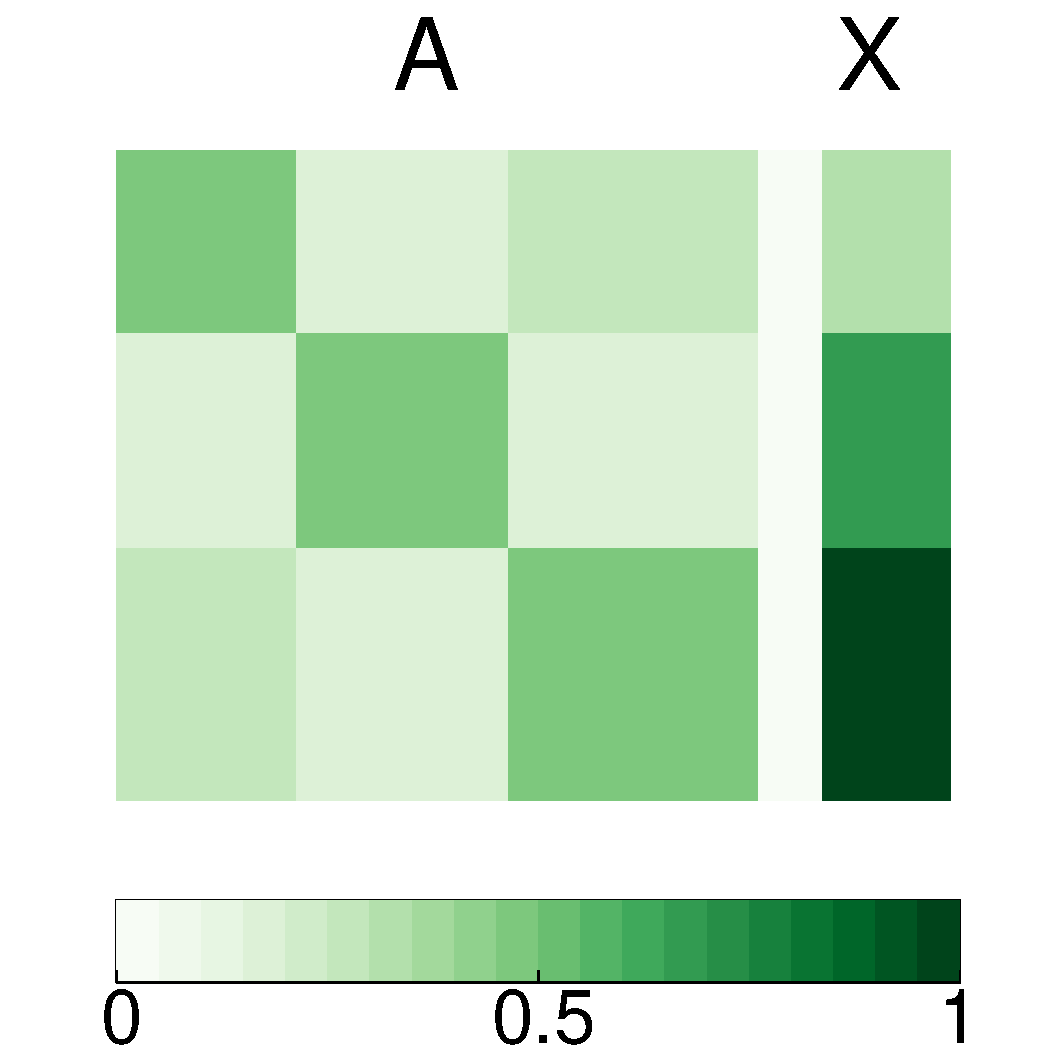
\includegraphics[width=\textwidth]{../Figure/Pmat.pdf}
		\caption{}
		\label{fig:a}
	\end{subfigure}
	~ %add desired spacing between images, e. g. ~, \quad, \qquad, \hfill etc. 
	%(or a blank line to force the subfigure onto a new line)
	\begin{subfigure}[b]{0.23\textwidth}
		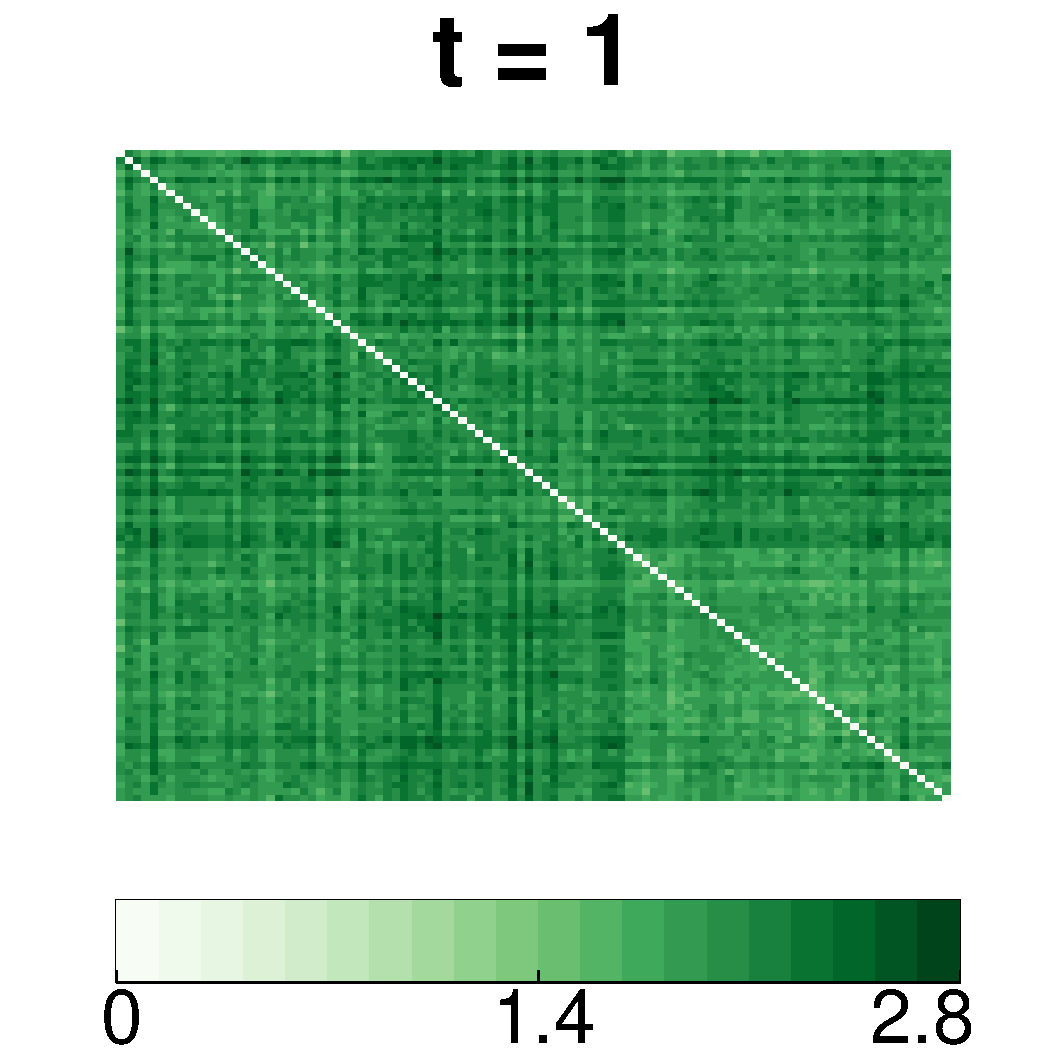
\includegraphics[width=\textwidth]{../Figure/Dx1.pdf}
		\caption{}
		\label{fig:b}
	\end{subfigure}
	~ %add desired spacing between images, e. g. ~, \quad, \qquad, \hfill etc. 
	%(or a blank line to force the subfigure onto a new line)
	\begin{subfigure}[b]{0.23\textwidth}
		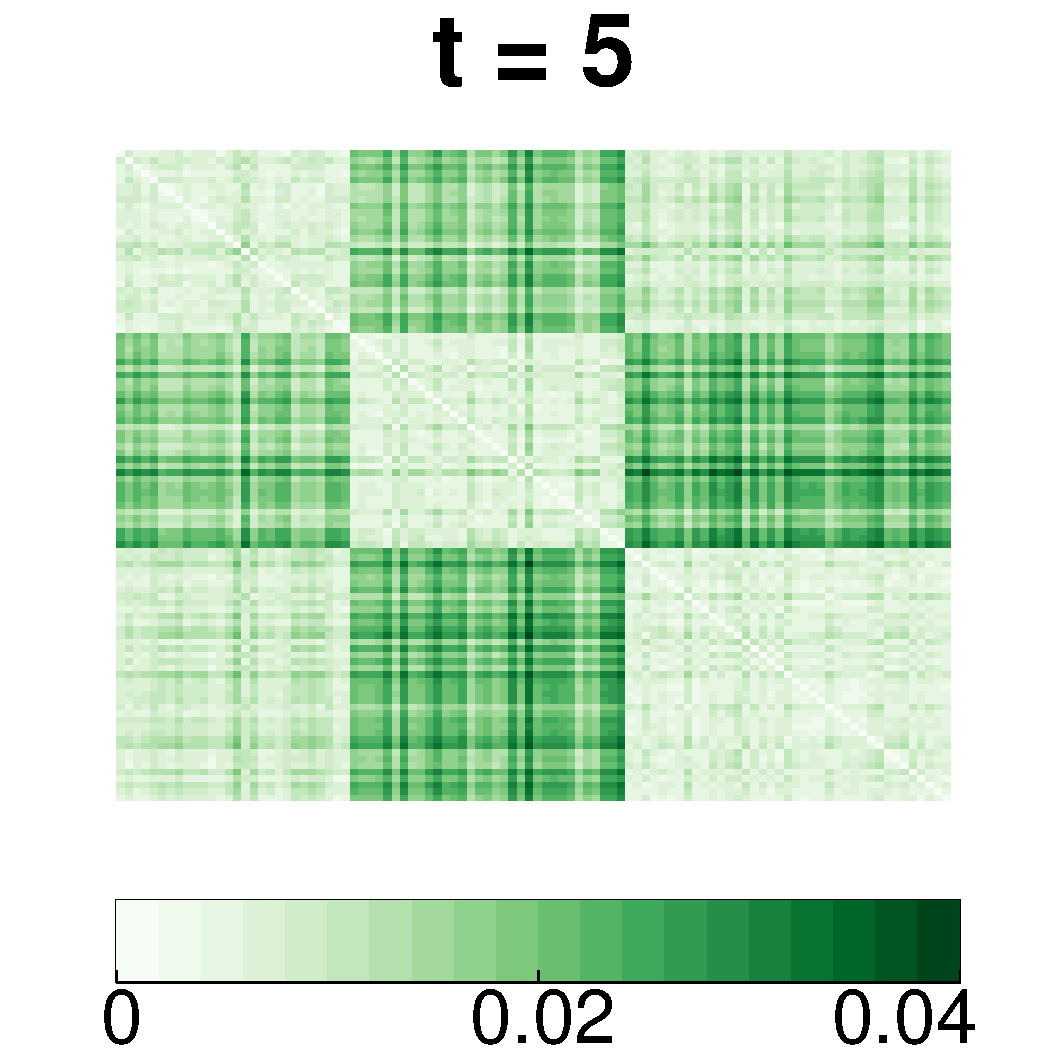
\includegraphics[width=\textwidth]{../Figure/Dx5.pdf}
		\caption{}
		\label{fig:c}
	\end{subfigure}
	\begin{subfigure}[b]{0.23\textwidth}
		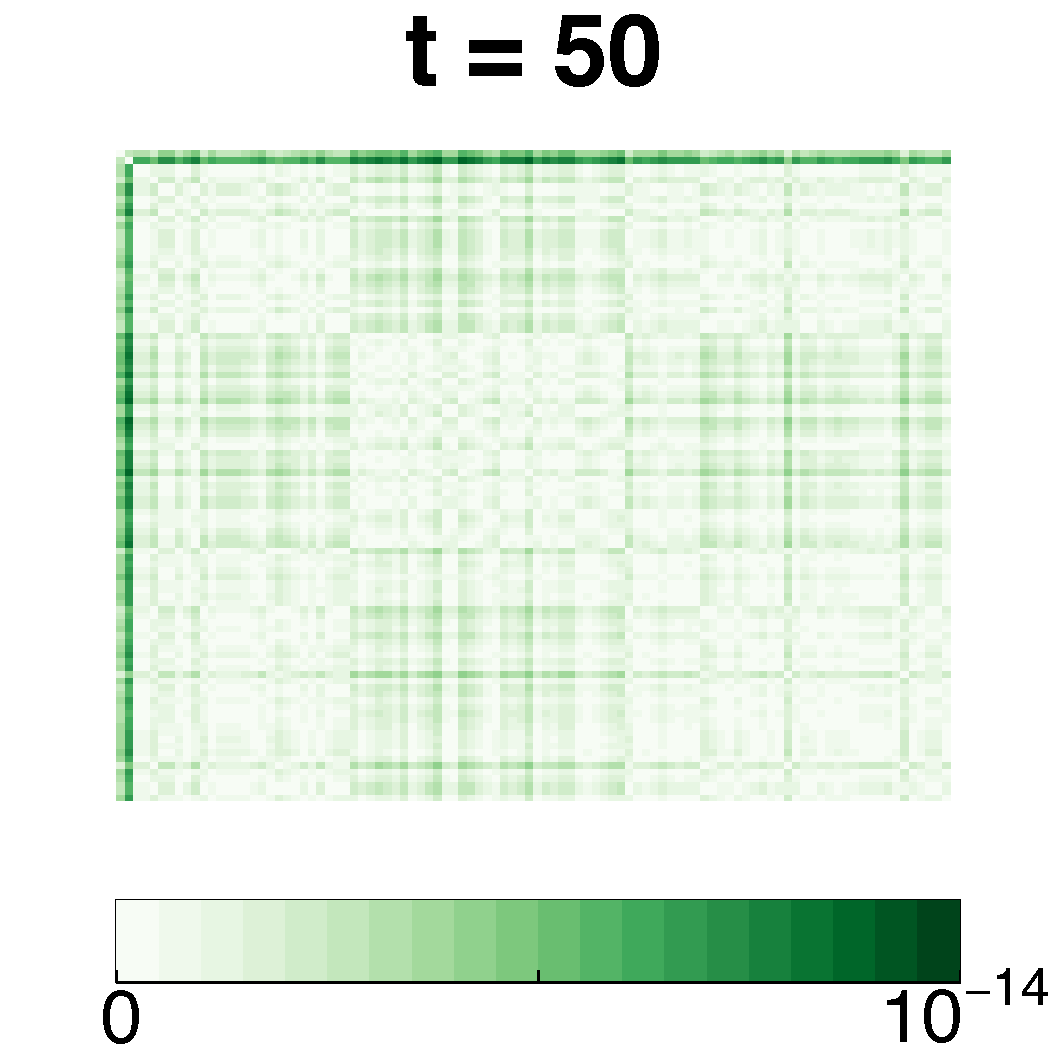
\includegraphics[width=\textwidth]{../Figure/Dx50.pdf}
		\caption{}
		\label{fig:d}
	\end{subfigure}
	\caption{Figure (a) shows data generating probability of adjacency matrix $\mathbf{A}$ and nodal attributes $\mathbf{X}$. Diffusion matrix, as a proposed network metrics, provides one-parameter family of network-based distances where as time goes by the pattern shown in the distance matrix changes, and at time point $t = 5$, distance matrix (c) illustrates most clear block structures and at the same time it exhibits most dependence to distance matrix of $\mathbf{X}$.}
	\label{fig:diffusions}
\end{figure}
\cite{coifman2006diffusion} proposed diffusion maps as a meaningful multiscale geometries which is defined by eigenvectors of Markov matrix constructed over a connected network. In the process of constructing such Markov matrix, we basically run random walks by iterating transition matrix and diffusion maps accordingly locates each node's position at each iteration time. Distance between each pair of nodes, defined as a \textit{diffusion distance}, then can be derived from an Euclidean distance of such diffusion maps. Each of diffusion distance, i.e.~$C_{t}$, can also be represented using a discrete set of real nonzero eigenvalues $\{ \lambda_{r} \}$ and eigenvectors $\{ \phi_{r}  \}$ of a transition matrix~\citep{coifman2006diffusion,lafon2006diffusion}. 
\begin{equation}
\label{eq:diffusion}
C^2_{t}[i,j]  :=   \parallel \mathbf{U}_{t}(i) - \mathbf{U}_{t}(j) \parallel   \quad i,j = 1,2, \ldots , n,
\end{equation}
where $\mathbf{U}_{t}(i) = \begin{pmatrix} \lambda^{t}_{1} \phi_{1}(i) & \lambda^{t}_{2} \phi_{2} (i)  & \ldots & \lambda^{t}_{q} \phi_{q}(i) \end{pmatrix}^{T} \in \mathbb{R}^{q}$ is a diffusion map at time $t$. As diffusion time $t$ increases, distance matrix $C_{t}$ is more likely to take into account distance between two nodes which are relatively difficult to reach each other. Figure~\ref{fig:diffusions} shows three exemplary distance matrices among whole one-parameter family of distance $\{ C_{t} : t \in \mathbb{N} \}$. Compared to adjacent relation or geodesic distance which are two extremes, diffusion distance well reflects the connectivity since it takes into account every possible path between the two nodes. We proved that each diffusion map provides \textit{i.i.d} multivariate coordinates for each node under jointly exchangeable graph. Lemma~\ref{main_lemma} below provides us with \textit{i.i.d} one-parameter family of $\{ \mathbf{U}_{t} \}_{t \in \mathbb{N}}$. This validates using diffusion maps in distance-based independence test, e.g. \texttt{dCorr} or \texttt{MGC}, as a distance matrix as claimed in the following Theorem~\ref{theorem2}. 
\begin{lemma}[Exchangeability and \textit{i.i.d} of diffusion maps $\mathbf{U}_{t}$]
	\label{main_lemma}
	Assume that a connected, undirected and unweighted graph $\mathbf{G}$ is an exchangeable random graph. Then its transition probability so thus diffusion maps at fixed time $t$ is also exchangeable, conditioned on underlying distribution of graph. Furthermore, by \textit{de Finetti's Theorem}, such diffusion maps at $t$, $\mathbf{U}_{t}(i) = \begin{pmatrix} \lambda^{t}_{1} \phi_{1}(i) & \lambda^{t}_{2} \phi_{2} (i)  & \ldots & \lambda^{t}_{q} \phi_{q}(i) \end{pmatrix}^{T}$, are conditionally \textit{i.i.d} given its underlying distribution.   
\end{lemma}
\begin{theorem}
	\label{theorem2}
	For $n$-pair of diffusion map and \textit{i.i.d} nodal attributes $\{ ( \mathbf{u}_{t}(i),  \mathbf{x}_{i}  ) : i =1,2, \ldots , n \}$ in a jointly exchangeable graph $\mathbf{G}$, we have $\mathbf{u}_{t}(i) \overset{i.i.d}{\sim} f_{U^{(t)}}$ and $\mathbf{x}_{i} \overset{i.i.d}{\sim} f_{\mathbf{X}}$ conditioned on underlying distribution of graph. 
	Then \texttt{MGC} is consistent in testing network independence with null of $H_{0}: f_{\mathbf{U}^{(t)} \cdot \mathbf{X}  }  = f_{\mathbf{U^{(t)}}} \cdot f_{\mathbf{X}}$. In particular, the consistency also holds for using the estimated latent network factors~\citep{fosdick2015testing} or an adjacency matrix of directed network as a distance matrix.
\end{theorem}

\subsection{Measure for Node Contribution}
On the other hand, some nodes often exert more reliance on their attributes than the others. Here we suggest the measure of node's contribution to detecting dependence as a byproduct of \texttt{MGC} statistic. Let $(k^{*}, l^{*})$ be the optimal neighborhood choice in distance matrix $(C, D)$ respectively. Denote the contribution of node $v \in V(G)$ to the testing statistic by  $c(\cdot) : v \rightarrow \mathbb{R}$
\begin{equation}
\label{contribution}
c(v) \propto \sum\limits_{j=1}^{n} \tilde{C}_{j v} \tilde{D}_{j v} I \big(  r (C_{j v}) \leq k^{*}  \big) I \big( r (D_{ j v }) \leq l^{*} \big), 
\end{equation}
which is proportional to $v^{th}$ column-sum of the pre-summed test statistic~\ref{eq:MGC}. Note that the deviation of non-negative \texttt{MGC} statistic from zero implies departure from the independence and also note that we truncate the correlation in \texttt{dCov} by column entry's rank. Thus $\tilde{C}_{jv} \tilde{D}_{jv}$ would not be truncated if node $j$ $(\in \{ 1,2, \ldots, n \} \setminus \{v \} )$ is important to node $v$ and its larger, positive value would contribute to ${\mathcal{V}^{*}_{n}}^2$ more. The statistic $c(v)$ comes out from these observations. 

%%%%%%%%%%%%%%%%%%%%%%%%%%%%%%%%%%%%%%%%%%%%%%%%%%
\section{Simulation Study}
\label{sec:simulation}
	\vspace*{-0.2cm}
In our simulation studies, we make a comparison between empirical testing power between \texttt{MGC} and \texttt{mCorr}, and network model-based test of Fosdick and Hoff (\texttt{FH})~\citep{fosdick2015testing}. We use type I error of $\alpha = 0.05$ and obtain p-values from each simulated network via permutation test. All the simulation models can be illustrated by joint distribution of adjacent matrix $\mathbf{A}$, nodal attributes $\mathbf{X}$, and latent variable $\mathbf{Z}$ that explains dependence structure between $\mathbf{A}$ and $\mathbf{X}$. You can find the detailed simulation models in the Appendix~\ref{ssec:models}. We introduced a popular network model of Stochastic Block Model (SBM) as our main simulated networks. To scrutinize our conjecture on better performance of local optimal scaled \texttt{MGC} over global scale of \texttt{mCorr}, we control the amount of \textit{nonlinear dependency} through changing the value of $\theta \in (0, 1)$ in the three block model~\ref{eq:mono}. When $\theta > 0.2$, linear dependency of edge distribution in $\mathbf{A}$ upon nodal attribute of $X$ is lost. If you see Figure~\ref{fig:powerplot}, power of \texttt{mCorr} starts to drop from $\theta = 0.2$ while that of \texttt{MGC} almost stays clam, which implies \texttt{MGC} is significantly more sensitive to nonlinear dependency compared to \texttt{mCorr}.  
\begin{figure}[h]
	\centering
	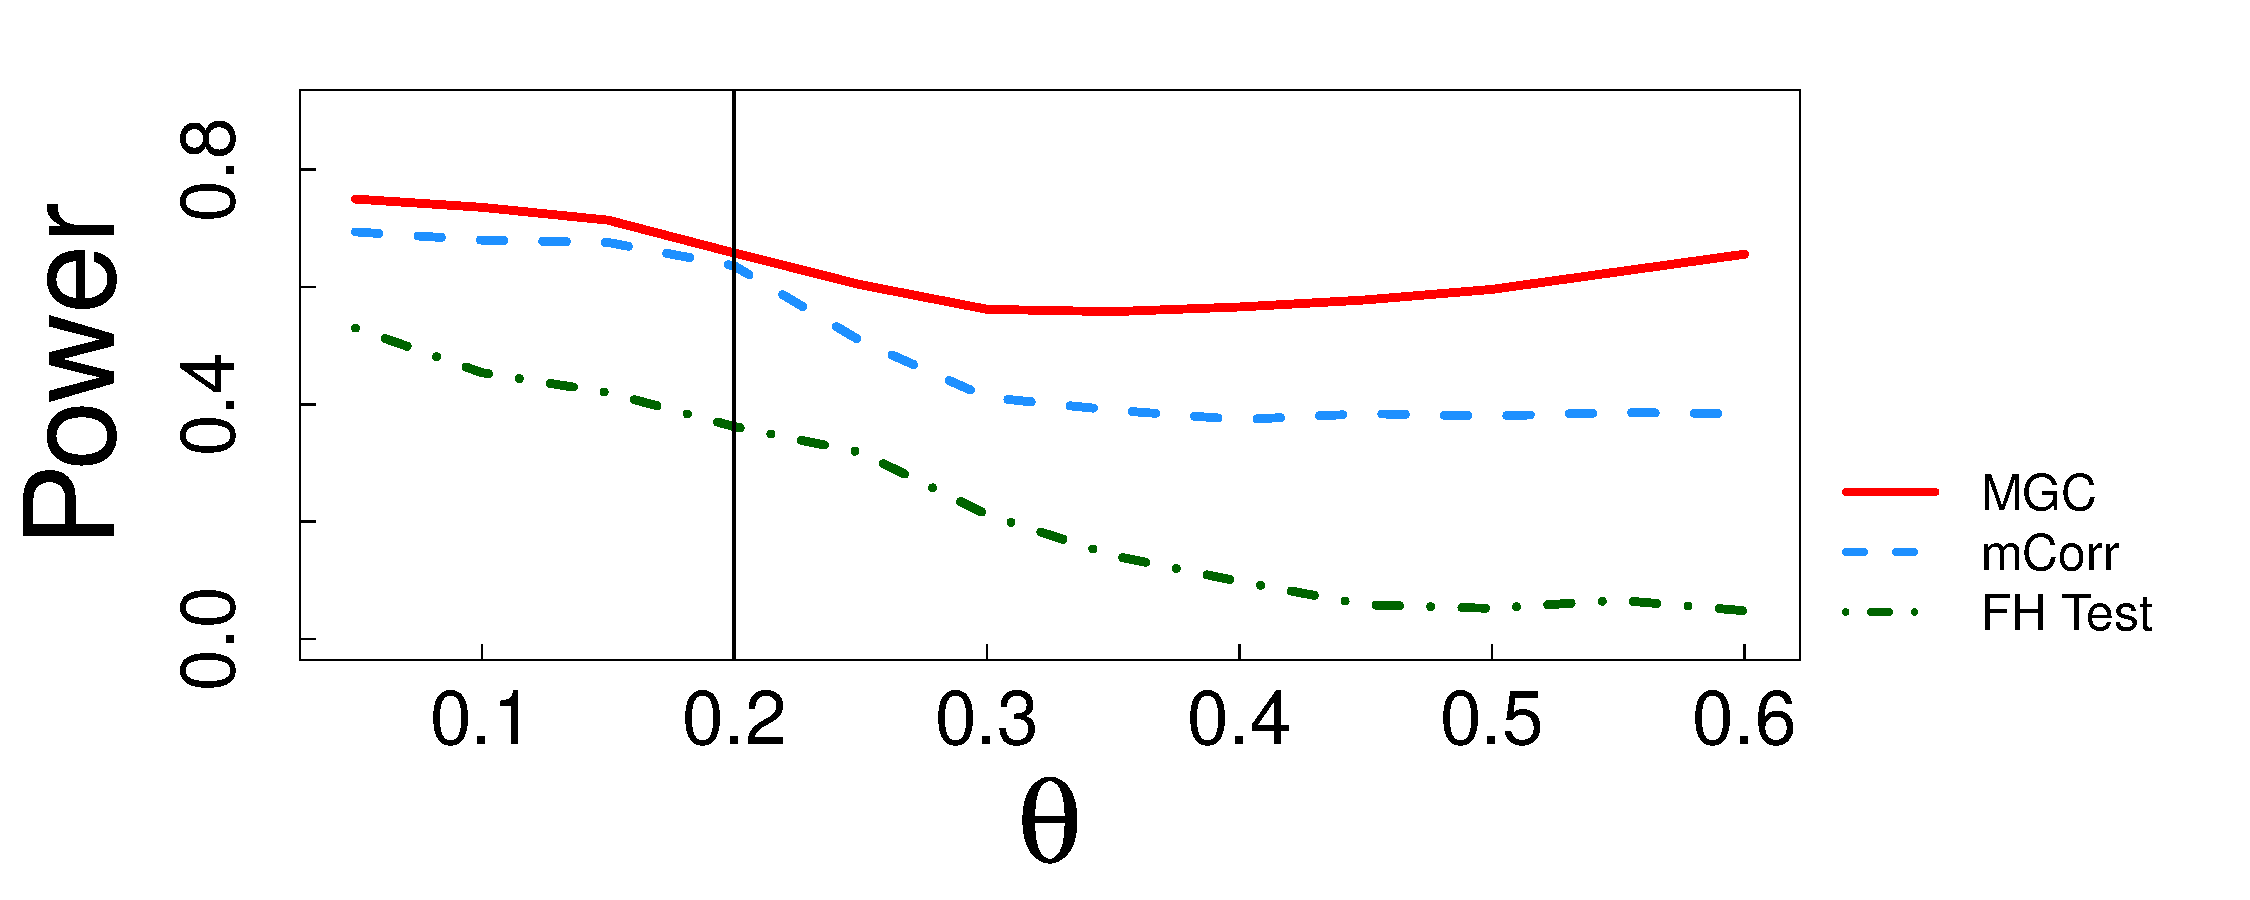
\includegraphics[width=0.7\linewidth]{../Figure/mono_simple.pdf}
	\caption{X-axis of $\theta$ controls the existence/amount of nonlinear dependency and in this particular case nonlinearity exists when $\theta > 0.2$ and gets larger as it increases. You can see the discrepancy in power between global and local scale tests also gets larger accordingly, mostly due to decreasing power of \texttt{mCorr} or \texttt{FH} test but relatively stable power of \texttt{MGC} under nonlinear dependency.}
	\label{fig:powerplot}
\end{figure}
	\vspace*{-0.4cm}
\begin{equation}
E(A_{ij} | X_{i}, X_{j}) = 0.5 I(|X_{i} - X_{j}| = 0) + 0.2 I(|X_{i} - X_{j}| = 1) + \theta I(|X_{i} - X_{j}| = 2)
\label{eq:mono}
	\vspace*{-0.4cm}
\end{equation}

% degree-corrected two block model
The SBM connotes that all nodes within the same block have the same expected degree. Thus, this block model is limited by homogeneous distribution within block and provides a poor fit to networks with highly varying node degrees within block or community. Instead the Degree-Corrected Stochastic Block model (DCSBM) proposed by \cite{karrer2011stochastic} add another random variable associated with each node to vary the node degrees. In the model~\ref{eq:dcVariance}, we controlled the amount of such variability by $\tau$; the larger the value $\tau$ is, the more variability degree or edge distribution has. In Figure~\ref{fig:dcSBM}, power based on Euclidean distance of $\mathbf{A}$ or that of estimated network factors (locations) becomes less sensitive as $\tau$ increases. Compared to these two, diffusion maps are more robust to such variability. 
\begin{figure}[h]
	\centering
	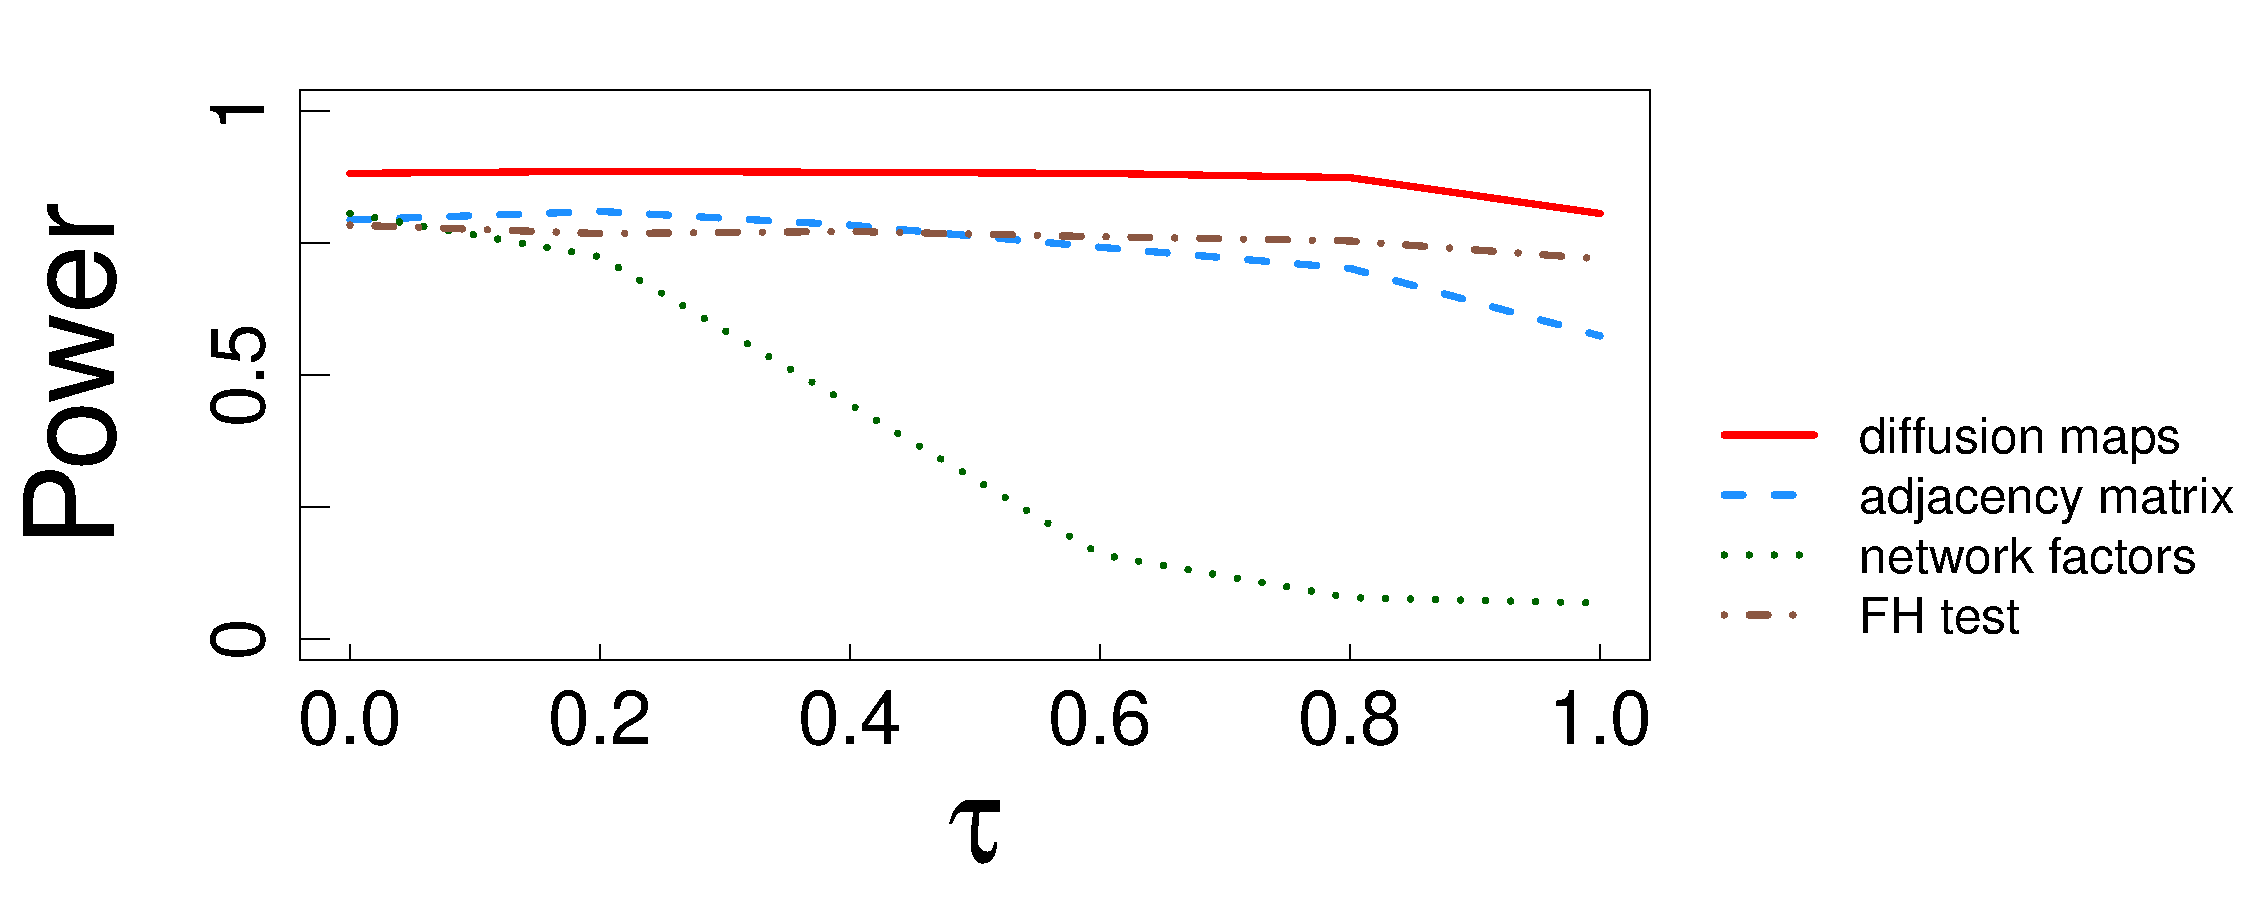
\includegraphics[width=0.7\linewidth]{../Figure/tau_simple.pdf}
	\caption{In degree-corrected SBM where the variability in degree distribution increases as $\tau$ increases, testing power of diffusion maps are more likely to be robust against increasing variability compared to other network metrics, e.g. adjacency matrix or latent positions. \texttt{FH} test statistics allowing different dimensions of network factors perform consistently well but still have less power than \texttt{MGC}.}
	\label{fig:dcSBM}
	\vspace*{-0.5cm}
\end{figure}	
\vspace*{-0.5cm}
\section{Conclusion}
\label{sec:conc}
	\vspace*{-0.2cm}
In this paper, we convince that \texttt{MGC}, merged with a family of diffusion distance, provides us powerful independence test statistics in network. Having multiscale statistics, i.e.~one parameter family of statistics, is not avoidable because we regard distance between nodes over network as a dynamic process. Through simulation studies, we demonstrated that our methods work better than the others especially under nonlinear dependency, and we are able to measure each node's contribution to detecting dependency. Deriving the contributions is particularly important when there have possibly different amounts of the dependencies among the nodes.  

However obtaining a full family of statistics are computationally infeasible. Also we did not suggest any theoretically supported tools to select one metrics among them so thus we have one single statistic. As an ad hoc, we selected an \textit{optimal} diffusion time $t$ with highest power from $t=1$ to $t=10$ for our simulation since we could observe a stabilized empirical power within this period. Developing the adaptive method to find this optimal $t$ where dependence is maximized would be a natural next step. Despite these shortcomings, we expect that we could also enjoy the properties of \texttt{MGC} and a family of diffusion distances in solving diverse problems which require to utilize local relationship of the data sets. For instance, we might be able to implement independence testing between two networks of same size by using diffusion distance of each network to investigate whether a pair of networks are topologically or structurally independent.

%%%%%%%%%%%%%%%%%%%%%%%%%%%%%%%%%%%%%%%%%%%%
\vspace*{-0.5cm}
\bibliography{reference}
%\bibliographystyle{plainnat}
%%%%%%%%%%%%%%%%%%%%%%%%%%%%%%%%%%%%%%%%%%%%%%
\vspace*{-0.5cm}
\section{Appendix}
\vspace*{-0.2cm}
\subsection{Lemmas and Theorems}
\label{ssec:proof}

%%%%%%%%%%%%%%%%%%%%%%%%%%%%%%%%%%%%%%%%	
\begin{proof}[\textbf{Proof of Lemma~\ref{main_lemma}}]
	Diffusion map at time $t$ is represented as follows :
	\begin{equation}
	\mathbf{U}_{t}(i) = \begin{pmatrix} \lambda^{t}_{1} \phi_{1}(i) & \lambda^{t}_{2} \phi_{2} (i)  & \cdots & \lambda^{t}_{q} \phi_{q}(i) \end{pmatrix} \in \mathbb{R}^{q}.
	\end{equation}
	where $\Phi = \Pi^{-1/2}\Psi$ and $Q= \Psi \Lambda \Psi^{T} = \Pi^{1/2} P \Pi^{-1/2}$. 
	Thus $P \Pi^{-1/2} \Psi = \Pi^{-1/2} \Psi \Lambda$. 
	Then for any $r$th row ($r \in \{1,2, ... , q \}$, $(q \leq n)$), we can see that $P \phi_{r} = \lambda_{r} \phi_{r}$  where $\phi_{r} = \begin{pmatrix}  \psi_{r}(1) / \sqrt{\pi(1)} &  \psi_{r}(2) /  \sqrt{\pi(2)} & \cdots & \psi_{r}(n) /  \sqrt{\pi(n)}  \end{pmatrix}$.
	Therefore to guarantee exchangeability (or \textit{i.i.d}) of $\mathbf{U}_{t}$, it suffices to show exchangeability (or \textit{i.i.d}) of $P$.
	
	Assume joint exchangeability of $\mathbf{G}$, i.e. $(A_{ij}) \stackrel{d}{=} \big( A_{\sigma(i) \sigma(j)} \big)$. Since $A_{ij}$ is binary, $A_{ij} / \sum\limits_{j} A_{ij} = A_{ij} /  (1 + \sum\limits_{l \neq j} A_{il})$. Moreover, $A_{ij}$ and $(1 + \sum\limits_{l \neq j} A_{il})$ are independent given its link function $g$, and $A_{\sigma(i) \sigma(j)}$ and $(1 + \sum\limits_{l \neq j} A_{\sigma(i) \sigma(l)})$ are independent also given $g$. Then the following joint exchangeability of transition probability holds for $i \neq j; i,j = 1,2, \ldots,n$:	
	\begin{equation}
		\vspace*{-0.2cm}
	\big( P_{ij} \big) = \left(  \frac{A_{ij}}{1 - A_{ij} + \sum\limits_{j=1}^{n} A_{ij} } \right)  \stackrel{d}{=} \left( \frac{A_{\sigma(i) \sigma(j)} }{1 - A_{\sigma(i) \sigma(j)} + \sum\limits_{\sigma(j) = 1}^{n} A_{\sigma(i) \sigma(j)} } \right) = \big( P_{\sigma(i) \sigma(j)} \big)
	\end{equation}
	When $i = j$, $P_{ij} = P_{\sigma(i) \sigma(j)} = 0$ for $i=1,2, \ldots, n$. Thus, transition probability is also exchangeable. This results exchangeable eigenfunctions $\{ \Phi(1), \Phi(2), , ... , \Phi(n) \}$ where $\Phi(i) := \begin{pmatrix} \phi_{1}(i) & \phi_{2}(i) & \cdots & \phi_{q}(i) \end{pmatrix}^{T}$, $i=1,2, \ldots, n$. Thus diffusion maps at fixed $t$, $\mathbf{U}_{t} = \begin{pmatrix} \Lambda^{t} \Phi(1)  & \Lambda^{t} \Phi(2) & \cdots & \Lambda^{t} \Phi(n)  \end{pmatrix}$ are exchangeable. Furthermore by \textit{de Finetti's Theorem}, we can say that $\mathbf{U}(t) = \{ \mathbf{U}_{t}(1), \mathbf{U}_{t}(2), \ldots, \mathbf{U}_{t}(n)    \}$ are conditionally independent on their underlying distribution.
\end{proof}

\begin{proof}[\textbf{Proof of Theorem~\ref{theorem2}} Consistency of \texttt{MGC} applied to exchangeable variables]
	
	Under the exchangeability and finite second moment assumptions of underlying distribution, $\mathcal{V}^{2}_{n}(\mathbf{X},\mathbf{Y}) \xrightarrow{n \rightarrow \infty}  0$ if and only if underlying distribution of $\{\mathbf{x}_{i} \}$, $f_{\mathbf{x}}$ is independent from underlying distribution of $\{ \mathbf{y}_{i}  \}$, $f_{\mathbf{y}}$. Now suppose that we have undirected, connected network $\mathbf{G}$ with a family of diffusion maps $\{ \mathbf{u}_{t}  \}$ and with nodal attributes $\{ \mathbf{x}  \}$. We have shown in the Lemma~\ref{main_lemma} that $\{ \mathbf{u}_{t}  \}$ are exchangeable for each $t \in \mathbb{N}$. Thus there exists an underlying distribution of $\mathbf{u}_{t}$ such that $\mathbf{u} \overset{i.i.d}{\sim} f_{\mathbf{u}^{(t)}}$ for $t= 1,2,\ldots $; and we have $\mathbf{x}_{i} \overset{i.i.d}{\sim} f_{\mathbf{X}}$. Under the assumption of finite second moment of $\mathbf{u}^{(t)}$ and $\mathbf{x}$, \texttt{MGC} statistics constructed by $\{  (  \mathbf{u}_{ti}, \mathbf{x}_{i} ) : i = 1,2,\ldots, n  \}$ yield a consistent testing which determines the independence between underlying distributions of $\mathbf{u}^{(t)}$ and $\mathbf{x}$. From the same setting of network $\mathbf{G}$, we have estimated \textit{i.i.d} node-specific network factors $\{ \mathbf{F}_{i} \}$ so that $n$-pair of \textit{i.i.d} $\{ ( \mathbf{F}_{i}, \mathbf{x}_{i} )  \}$ can be applied to \texttt{MGC} or other distance-based tests without assuming conditioning underlying distribution. In case of using adjacency matrix directly into test, we must assume that the adjacency matrix comes from connected directed network, i.e. $A_{ij} \overset{i.i.d}{\sim} f_{A}$ for all $i,j=1,2,\ldots, n$; otherwise, each column is dependent on one another.  
\end{proof}

\subsection{Simulation Data}
\label{ssec:models}

\begin{itemize}	
	\item \textbf{Three Block SBM} $(n = 100)$
	\vspace*{-0.5cm}
	\begin{equation}
	\label{eq:Three}
	\begin{gathered}
	\begin{aligned}
	&  X_{i} \overset{i.i.d}{\sim} f_{X}(x)   \stackrel{d}{=}  Multi(1/3, 1/3, 1/3), i = 1, \ldots , n \\ 
	&  Z_{i} | X_{i}  \overset{i.i.d}{\sim}    f_{Z|X}(z|x)  \stackrel{d}{=}   Multi(0.5, 0.25, 0.25) I( x = 1 ) +   Multi(0.25, 0.5, 0.25) I (x = 2)  \qquad  \\ & \quad \quad + Multi(0.25, 0.25, 0.5)I(x = 3), \quad  i = 1,\ldots,n  \\
	&  A_{ij} | Z_{i}, Z_{j}   \overset{i.i.d}{\sim}   f_{A|Z}(a_{ij} | z_{i}, z_{j}) \stackrel{d}{=}  Bern(0.5) I ( |z_{i} - z_{j}| = 0 )  + Bern(0.2) I(|z_{i} - z_{j}| = 1) \\ & \quad \quad + Bern(0.3) I (|z_{i} - z_{j}| = 2),  \quad i < j, i,j=1, \ldots n 
	\end{aligned}
	\end{gathered}
	\end{equation}
	\vspace*{-1.5cm}
	\item \textbf{Increasing variance in DCSBM} $(n = 250)$
	\vspace*{-0.5cm}
	\begin{equation}
	\label{eq:dcVariance}
	\begin{gathered}
	\begin{aligned}
	&  X_{i} \overset{i.i.d}{\sim} f_{X}(x)   \stackrel{d}{=}  Bern(0.5), \quad i = 1, \ldots , n \\ 
	&  Z_{i} | X_{i}  \overset{i.i.d}{\sim}    f_{Z|X}(z|x)  \stackrel{d}{=}   Bern(0.6) I( x = 0 ) + Bern(0.4) I (x = 1) \quad  i = 1,\ldots,n  \\
	& \theta_{i} \overset{i.i.d}{\sim} Uniform(1 - \tau, 1 + \tau), i = 1, \ldots, n; \quad \tau = 0, 0.2, \ldots, 1\\ 
	& A_{ij} | \mathbf{Z}, \mathbf{\theta}   \overset{i.i.d}{\sim}   f_{A|Z, \theta}(a_{ij} | z_{i}, z_{j}, \theta_{i}, \theta_{j}) \stackrel{d}{=} Bern(0.2 \cdot \theta_{i}\theta_{j}) I ( |z_{i} - z_{j}| = 0 ) \\ & \quad \quad + Bern(0.05 \cdot \theta_{i} \theta_{j} ) I(|z_{i} - z_{j}| = 1), \quad i,j=1, \ldots, n; i < j. 
	\end{aligned}
	\end{gathered}
	\end{equation}
	
\end{itemize}

\end{document}